% !TEX root = thesis.tex
\chapter{Background}
\label{sec:background}

This chapter introduces the theoretical and technical background required for the design and implementation presented in this thesis. It first describes the fundamental principles of Spiking Neural Networks and the Leaky Integrate-and-Fire neuron model. It then reviews the main learning approaches for \gls{snn}s and introduces the Spike-Driven Synaptic Plasticity rule in detail. The final sections present the concepts of \gls{fpga}-based neural-network acceleration and Dynamic Partial Reconfiguration required for the later design assessment, followed by the Spiker+ framework on which the implemented accelerator is based.

\section{Spiking Neural Networks}
\label{subsec: spiking neural networks}

\gls{snn}s are a class of biologically inspired neural networks that process and transmit information through discrete events known as spikes \cite{Maass1997,Gerstner2014}. They are commonly described as the third generation of \gls{ann}s. In traditional \gls{ann}s, neurons generally receive continuous-valued inputs, calculate a weighted sum, and apply an activation function to produce a continuous-valued output \cite{Maass1997}. In contrast, a spiking neuron maintains an internal state that evolves over time and generates an output spike only when a firing condition is satisfied. Therefore, \gls{snn}s introduce an explicit temporal dimension into neural information processing.

An \gls{snn} generally consists of interconnected spiking neurons and synapses \cite{Gerstner2014}. Each synapse connects a presynaptic neuron to a postsynaptic neuron and is associated with a synaptic weight. When a presynaptic spike arrives, it changes the internal state of the postsynaptic neuron according to the corresponding weight. Excitatory synapses increase the likelihood that the postsynaptic neuron will fire, whereas inhibitory synapses reduce it. The neuron integrates these synaptic events over time and produces an output spike when its membrane potential reaches a defined threshold.

\begin{figure}[t]
	\centering
	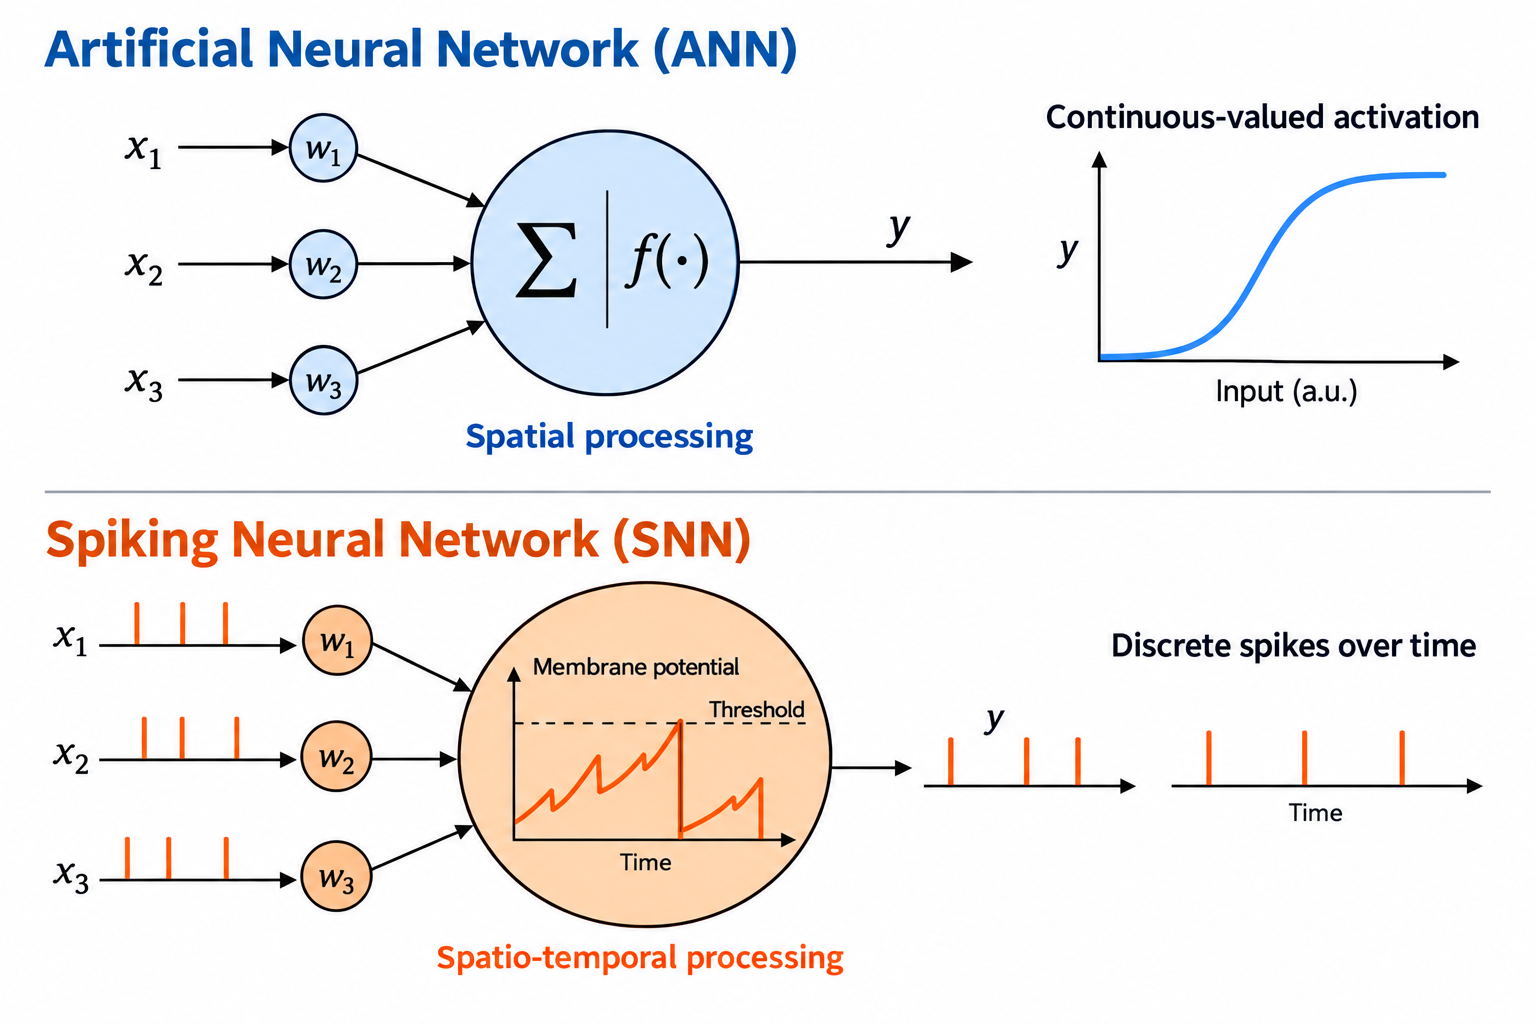
\includegraphics[width=.9\linewidth]{figures/ann_snn_comparison.png}
	\caption{Comparison of Information Processing in Artificial and Spiking Neurons}
	\label{fig:ann_snn_comparison}
\end{figure}

Figure \ref{fig:ann_snn_comparison} illustrates the main conceptual differences between a traditional artificial neuron and a spiking neuron. In an \gls{ann}, the weighted inputs are combined and transformed by an activation function, producing a continuous-valued output. The computation is mainly determined by the values presented to the neuron during a processing step. In an \gls{snn}, the inputs and outputs are represented by spike events distributed over time. Incoming spikes modify the membrane potential, which accumulates and gradually decays. When the membrane potential reaches the firing threshold, the neuron generates an output spike and its state is reset. Consequently, the behaviour of a spiking neuron depends not only on the presence of input events but also on their timing and the previous state of the neuron.

This distinction is often described as spatial processing in traditional \gls{ann}s and spatio-temporal processing in \gls{snn}s \cite{Maass1997}. The synaptic weights describe the spatial relationships between connected neurons, while the timing of spikes provides an additional temporal component. This does not imply that traditional neural networks cannot process temporal data. Instead, the difference concerns the fundamental communication mechanism and the explicit internal dynamics of the neuron model.

Information in an \gls{snn} can be encoded in several ways. In rate-based encoding, a larger input value is generally represented by a larger number of spikes within a defined time interval \cite{Gerstner2014}. In temporal encoding, information is represented by characteristics such as the time of the first spike or the relative timing between spikes \cite{Thorpe2001}. The selected encoding method influences the processing latency, spike activity, and complexity of the hardware implementation.

\gls{snn}s can be organized using network structures similar to those of traditional neural networks. For example, a feedforward \gls{snn} transfers spikes from an input layer through one or more processing layers to an output layer. Recurrent connections may also be included to preserve temporal information and model dynamic behaviour. In a classification task, the input data are first converted into spike trains and applied to the input neurons. The spikes propagate through weighted synapses to the output neurons, and the predicted class can be determined from their firing activity, for example, by identifying the neuron that produces the largest number of spikes during the observation period.

A major characteristic of \gls{snn}s is their event-driven operation \cite{Davis2018,Maass1997}. Computation is mainly triggered by the arrival of spikes rather than being performed continuously for every neuron and synapse. If spike activity is sufficiently sparse, inactive parts of the network do not need to perform synaptic operations \cite{Davis2018}. This property can reduce the number of computations and memory accesses. However, these potential advantages depend strongly on the network architecture, spike-encoding method, activity level, and hardware implementation. An inefficient implementation may not benefit from the sparsity of the spike events.

The event-driven and parallel characteristics of \gls{snn}s make them suitable for specialized hardware platforms \cite{Carpegna2025}. Neuromorphic processors, \gls{asic}s, and \gls{fpga}s can exploit parallelism between neurons and process spike events with deterministic latency. \Glspl{fpga} are particularly useful for \gls{snn} research because their configurable logic and memory resources allow different neuron models, numerical representations, and network structures to be implemented and evaluated without manufacturing a dedicated chip \cite{Carpegna2022}.

Despite their potential advantages, \gls{snn}s also present several challenges. Their temporal behaviour makes training and evaluation more complex than for traditional \gls{ann}s. Spike generation is non-differentiable, which prevents the direct application of standard gradient-based training methods without approximation. Hardware implementations must additionally manage neuron states, spike timing, synaptic memory, and communication between neurons. Supporting online learning further increases the complexity because synaptic weights must be updated during network operation instead of remaining fixed after offline training.

Therefore, the choice of neuron model and learning rule has an important effect on the computational complexity and hardware requirements of an \gls{snn}. Simplified neuron models are commonly used to retain the essential temporal behaviour of biological neurons while reducing implementation cost. The following sections introduce the spiking-neuron model and learning principles used as the theoretical basis of this work.

\section{Spiking Neuron Models}
\label{subsec: spiking neuron models}

Spiking-neuron models describe how neurons receive input spikes, update their internal states, and generate output spikes. Different models provide different levels of biological accuracy and computational complexity. The Hodgkin--Huxley model describes biological ion-channel dynamics in detail but requires several nonlinear differential equations \cite{HodgkinHuxley1952}. The Izhikevich model is computationally simpler while reproducing various biological firing patterns \cite{Izhikevich2003}. For digital hardware implementations, simplified models such as the \gls{if} and \gls{lif} models are more commonly used \cite{Gerstner2014}.

The \gls{lif} model provides a suitable compromise between biological plausibility and implementation efficiency. Its main state variable is the membrane potential \(V(t)\), which represents the electrical state of the neuron. Incoming spikes change the membrane potential according to their synaptic weights. In the absence of input, the membrane potential gradually returns towards its resting value. This behaviour is referred to as membrane leakage.

The membrane-potential dynamics of an \gls{lif} neuron are described by \cref{eq:lif-membrane-dynamics} \cite{Gerstner2014}.

\begin{equation}
    \tau_m \frac{\mathrm{d}V(t)}{\mathrm{d}t}
    =
    -\left(V(t)-V_{\mathrm{rest}}\right)
    + R_m I(t)
    \label{eq:lif-membrane-dynamics}
\end{equation}

where \(\tau_m\) is the membrane time constant, \(V_{\mathrm{rest}}\) is the resting potential, \(R_m\) is the membrane resistance, and \(I(t)\) represents the total input current. The leakage term causes the membrane potential to decay over time, while the input current term increases or decreases it in response to synaptic events.

The total synaptic input is determined by the received presynaptic spikes and their associated weights, as shown in \cref{eq:total-input-current} \cite{Gerstner2014}.

\begin{equation}
    I(t)
    =
    \sum_{i} w_i s_i(t)
    \label{eq:total-input-current}
\end{equation}

where \(w_i\) is the weight of synapse \(i\), and \(s_i(t)\) indicates the occurrence of a presynaptic spike. Excitatory synapses increase the membrane potential, whereas inhibitory synapses decrease it. Because spikes can be represented as binary events, synaptic processing can often be implemented using additions and subtractions rather than general multiplication operations.

\begin{figure}[t]
	\centering
	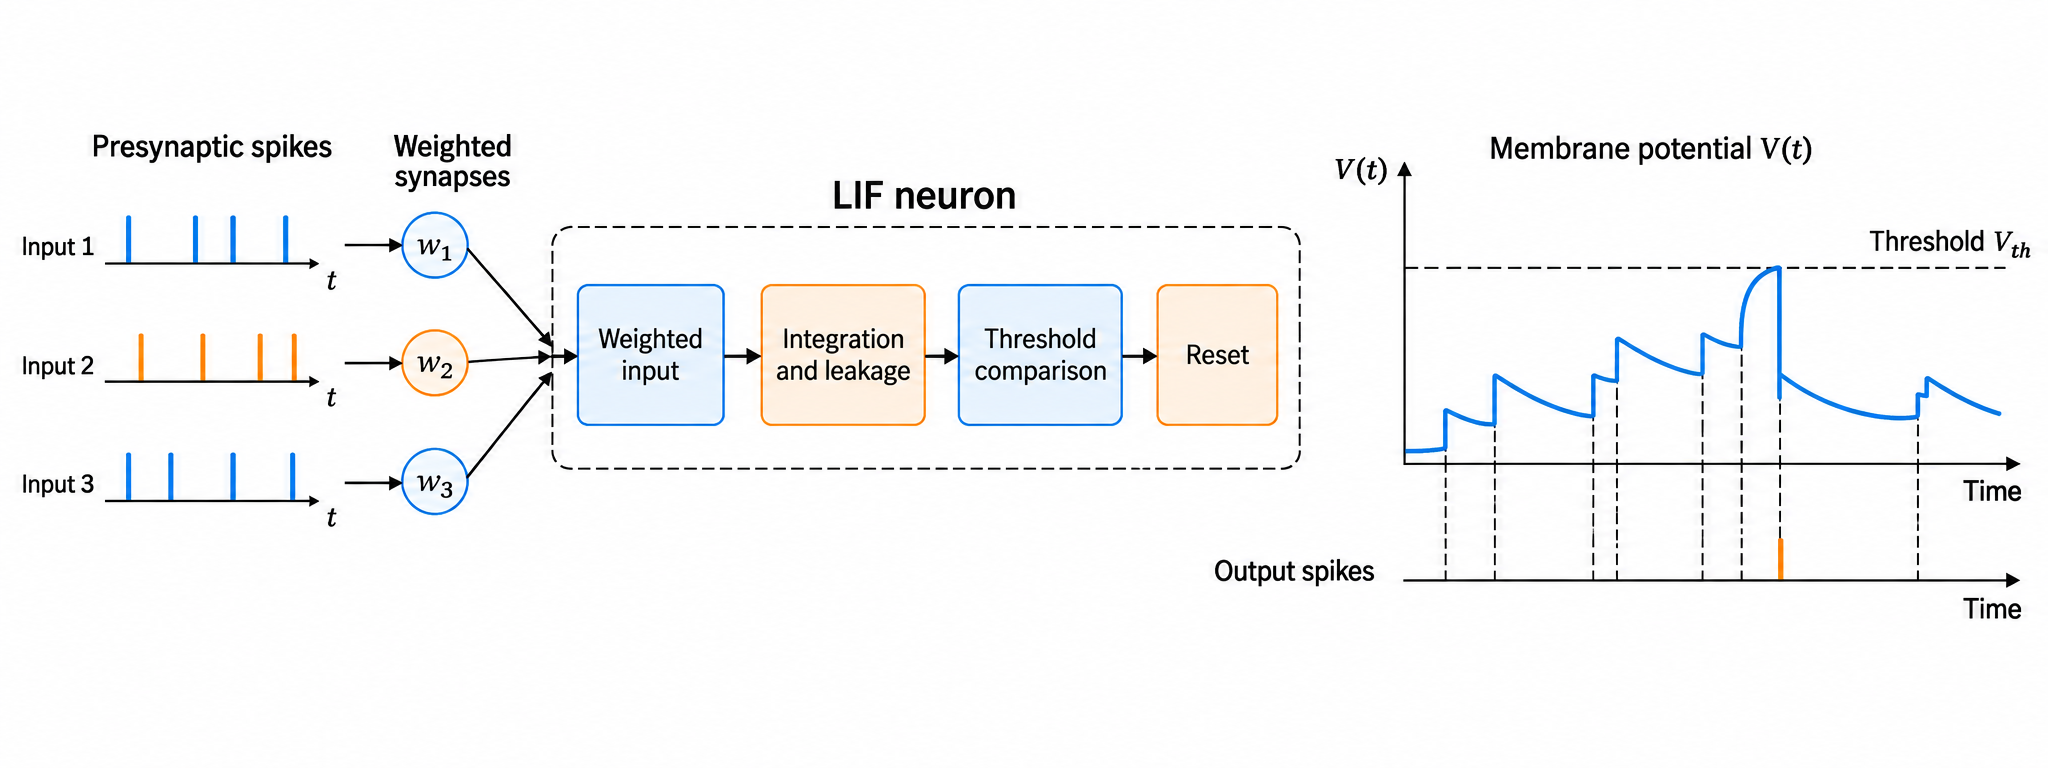
\includegraphics[width=.98\linewidth]{figures/lif_neuron_model.png}
	\caption{\gls{lif} Neuron Model Operating Principle}
	\label{fig:lif-neuron-model}
\end{figure}

Figure \ref{fig:lif-neuron-model} illustrates the operating principle of the \gls{lif} neuron model. Each presynaptic spike produces a weighted change in the membrane potential. Between input events, the potential decreases because of leakage. When several input spikes arrive within a sufficiently short interval, their effects accumulate and may cause the membrane potential to reach the firing threshold \(V_{\mathrm{th}}\). The output of the neuron can be represented as

\begin{equation}
    s_{\mathrm{out}}(t)
    =
    \begin{cases}
        1, & V(t) \geq V_{\mathrm{th}} \\
        0, & V(t) < V_{\mathrm{th}}
    \end{cases}
    \label{eq:output-spike-generation}
\end{equation}

After an output spike is generated, the neuron state must be reset. In a hard-reset model, the membrane potential is directly set to a predefined reset value. In a subtractive-reset model, the firing threshold is subtracted from the membrane potential:

\begin{equation}
    V(t) \leftarrow V(t) - V_{\mathrm{th}}
    \label{eq:subtractive-reset}
\end{equation}

Unlike a hard reset, the subtractive reset preserves the portion of the membrane potential that exceeds the firing threshold \cite{Rueckauer2017}. This remaining potential can contribute to subsequent spike generation. A refractory period may also be introduced to prevent the neuron from firing again immediately after an output spike.

For implementation in synchronous digital hardware, the continuous-time equation is converted into a discrete-time form. A simplified representation is

\begin{equation}
    V[k+1]
    =
    \alpha V[k]
    +
    \sum_{i} w_i s_i[k]
    \label{eq:discrete-membrane-update}
\end{equation}

where \(k\) denotes the current time step and \(\alpha\) is a decay factor representing membrane leakage. After the membrane potential is updated, it is compared with the firing threshold. If the threshold is reached, an output spike is generated and the reset operation is applied.

This discrete formulation mainly requires registers, adders, comparators, and simple leakage logic, making the \gls{lif} model well suited to \gls{fpga} implementation \cite{Carpegna2025}. Fixed-point or integer arithmetic can be used instead of floating-point arithmetic to reduce hardware complexity. The selected bit width and numerical precision influence both the accuracy of the neuron dynamics and the required hardware resources.

In this work, an \gls{lif} neuron model with subtractive reset is used as the processing element of the \gls{snn}. In addition to determining the generation of output spikes, its membrane potential is used by the \gls{sdsp} learning rule to control synaptic weight updates, which will be introduced in the following sections.

\section{Learning in Spiking Neural Networks}
\label{subsec: learning in spiking neural networks}

Learning enables an \gls{snn} to adapt its synaptic weights according to input data, neuronal activity, or external feedback. During inference, synaptic weights remain fixed and the network only processes incoming spikes. During learning, the weights are modified so that the network can adapt its response to particular input patterns. Because \gls{snn}s process information through discrete spikes and time-dependent neuron states, their learning mechanisms must consider not only neuronal activation but also the timing and sequence of spike events \cite{Gerstner2014,Neftci2019}.

This section first introduces the main learning approaches used in \gls{snn}s. It then focuses on \gls{sdsp}, which is the local online learning rule implemented in this work.

\subsection{Learning Approaches for Spiking Neural Networks}
\label{subsec: learning approaches for snns}

\gls{snn} learning methods can first be classified according to whether weight adaptation is performed offline or online. In offline learning, the network is trained before being deployed on the target hardware. Training can therefore be performed using \gls{cpu} or \gls{gpu}, and the resulting weights are subsequently transferred to the hardware accelerator. During normal hardware execution, these weights remain fixed. This approach avoids the additional control logic and writable weight storage required for training, but it prevents the deployed system from independently adapting to new data or changing operating conditions.

In online learning, synaptic weights are updated while the \gls{snn} is operating. The learning rule is evaluated directly from the observed network activity, allowing the system to adapt after deployment. However, the relevant neuron states must be available to the learning circuit, and inference and learning operations must be coordinated when accessing the same synaptic memory \cite{Frenkel2019ODIN}.

Learning methods can also be classified according to the source of the learning signal. In supervised learning, the desired output or class label is known during training, and the difference between the observed and desired output is used to guide the weight updates. In unsupervised learning, no explicit target output is available. Instead, synaptic weights are modified according to statistical patterns or correlations in the neuronal activity. Reinforcement learning uses a reward or penalty to evaluate the behaviour of the network without specifying the desired activity of every individual neuron \cite{Neftci2019}.

These classifications describe different aspects of the learning process and should not be considered mutually exclusive. For example, supervised learning may be performed offline using a gradient-based training algorithm or online using a teacher signal. Similarly, an unsupervised local rule may be implemented directly in hardware or simulated offline during network development.

Traditional \gls{ann}s are commonly trained using backpropagation and gradient descent. Applying these methods directly to \gls{snn}s is difficult because the spike-generation function is discontinuous. For a deterministic spiking neuron, its derivative is zero almost everywhere and undefined at the firing threshold. Consequently, the standard gradient cannot be propagated directly through the spike function. Surrogate-gradient methods address this problem by replacing the derivative of the spike function with a smooth approximation during training \cite{Neftci2019}. Such methods can train multilayer \gls{snn}s effectively, but they generally require error propagation and the storage of intermediate neuron states, which complicates direct online hardware implementation \cite{Zenke2018}.

Local learning rules provide an alternative approach. A local rule updates a synaptic weight using information that is available at or close to the corresponding synapse. This information may include presynaptic spikes, postsynaptic spikes, membrane potential, or a local activity trace. Because a complete error gradient does not need to be propagated through the network, local rules can reduce communication and memory requirements.

\gls{stdp} is a well-known example of local synaptic learning. In its basic form, the direction of the weight change depends on the relative timing of presynaptic and postsynaptic spikes. A presynaptic spike occurring shortly before a postsynaptic spike commonly causes synaptic potentiation, whereas the opposite order commonly causes synaptic depression \cite{BiPoo1998}. Evaluating \gls{stdp} requires information about the timing difference between the two spike events.

For resource-constrained online-learning hardware, local rules that require only a small number of neuron-state variables are particularly attractive. \gls{sdsp} follows this principle by triggering weight-update decisions on presynaptic spike events and determining the update direction from the current postsynaptic neuron state \cite{Brader2007}. The rule is described in detail in Section \ref{subsec: sdsp}.

\subsection{Spike-Driven Synaptic Plasticity}
\label{subsec: sdsp}

\gls{sdsp} was introduced by Brader, Senn, and Fusi as a local learning mechanism for networks that learn temporal spike patterns \cite{Brader2007}. The rule was designed so that synaptic updates depend only on information locally available at the synapse and the postsynaptic neuron. It therefore avoids the backward propagation of a global error signal and is suitable for event-driven online learning.

An \gls{sdsp} update is evaluated when a presynaptic spike arrives. At that moment, the rule observes the postsynaptic membrane potential and a calcium-related activity variable. The membrane potential describes the current state of the postsynaptic neuron, while the calcium variable provides an estimate of its recent firing activity. These two variables determine whether the active weight should be increased, decreased, or left unchanged \cite{Brader2007,Frenkel2019ODIN}.

The calcium variable \(C(t)\) can be represented as an activity trace that increases when the postsynaptic neuron produces a spike and decreases over time. A general continuous-time representation is

\begin{equation}
    \frac{\mathrm{d}C(t)}{\mathrm{d}t}
    =
    -\frac{C(t)}{\tau_C}
    +
    J_C \sum_{k}
    \delta\left(t-t_k^{\mathrm{post}}\right)
    \label{eq:calcium-dynamics}
\end{equation}

where \(\tau_C\) is the calcium decay time constant, \(J_C\) is the increase caused by a postsynaptic spike, and \(t_k^{\mathrm{post}}\) denotes the occurrence time of the \(k\)-th postsynaptic spike \cite{Brader2007}. Consequently, a high calcium value indicates strong recent postsynaptic activity, whereas a low value indicates limited activity.

In a digital implementation, the continuous calcium variable can be approximated using a counter. The counter is incremented when a postsynaptic spike occurs and decremented when a leakage event is received. This replaces continuous decay with discrete state updates and avoids the need for complex arithmetic. The calcium value is then compared with a set of programmable thresholds \cite{Frenkel2019ODIN}.

A commonly used hardware-oriented formulation of the \gls{sdsp} update rule can be expressed as

\begin{equation}
    \Delta w
    =
    \begin{cases}
        +1,
        & V_{\mathrm{mem}}\left(t_{\mathrm{pre}}\right) > \theta_m
          \ \text{and}\
          \theta_1 < C\left(t_{\mathrm{pre}}\right) < \theta_3
        \\[2pt]
        -1,
        & V_{\mathrm{mem}}\left(t_{\mathrm{pre}}\right) \leq \theta_m
          \ \text{and}\
          \theta_1 < C\left(t_{\mathrm{pre}}\right) < \theta_2
        \\[2pt]
        0,
        & \text{otherwise}
    \end{cases}
    \label{eq:sdsp-weight-update}
\end{equation}

where \(t_{\mathrm{pre}}\) is the arrival time of the presynaptic spike, \(V_{\mathrm{mem}}\) is the postsynaptic membrane potential, \(\theta_m\) is the membrane-potential threshold, and \(\theta_1\), \(\theta_2\), and \(\theta_3\) are calcium thresholds with \(\theta_1 < \theta_2 < \theta_3\) \cite{Frenkel2019ODIN}.

When the membrane potential is above \(\theta_m\), the postsynaptic neuron is considered sufficiently activated. If the calcium value is also within the potentiation interval, the synaptic weight is increased. When the membrane potential is below or equal to \(\theta_m\) and the calcium value is within the depression interval, the weight is decreased. In all other cases, the weight remains unchanged.

The calcium thresholds prevent learning when the postsynaptic neuron is either insufficiently active or excessively active. The lower threshold \(\theta_1\) prevents updates when the recent postsynaptic activity is too low. The upper thresholds \(\theta_2\) and \(\theta_3\) define the activity ranges in which depression and potentiation are permitted. This behaviour acts as a stop-learning mechanism and limits continuous weight modification outside the desired activity range \cite{Brader2007}.

Figure \ref{fig:conceptual-operation-of-sdsp} summarizes the information flow of the \gls{sdsp} learning rule.

\begin{figure}[t]
	\centering
	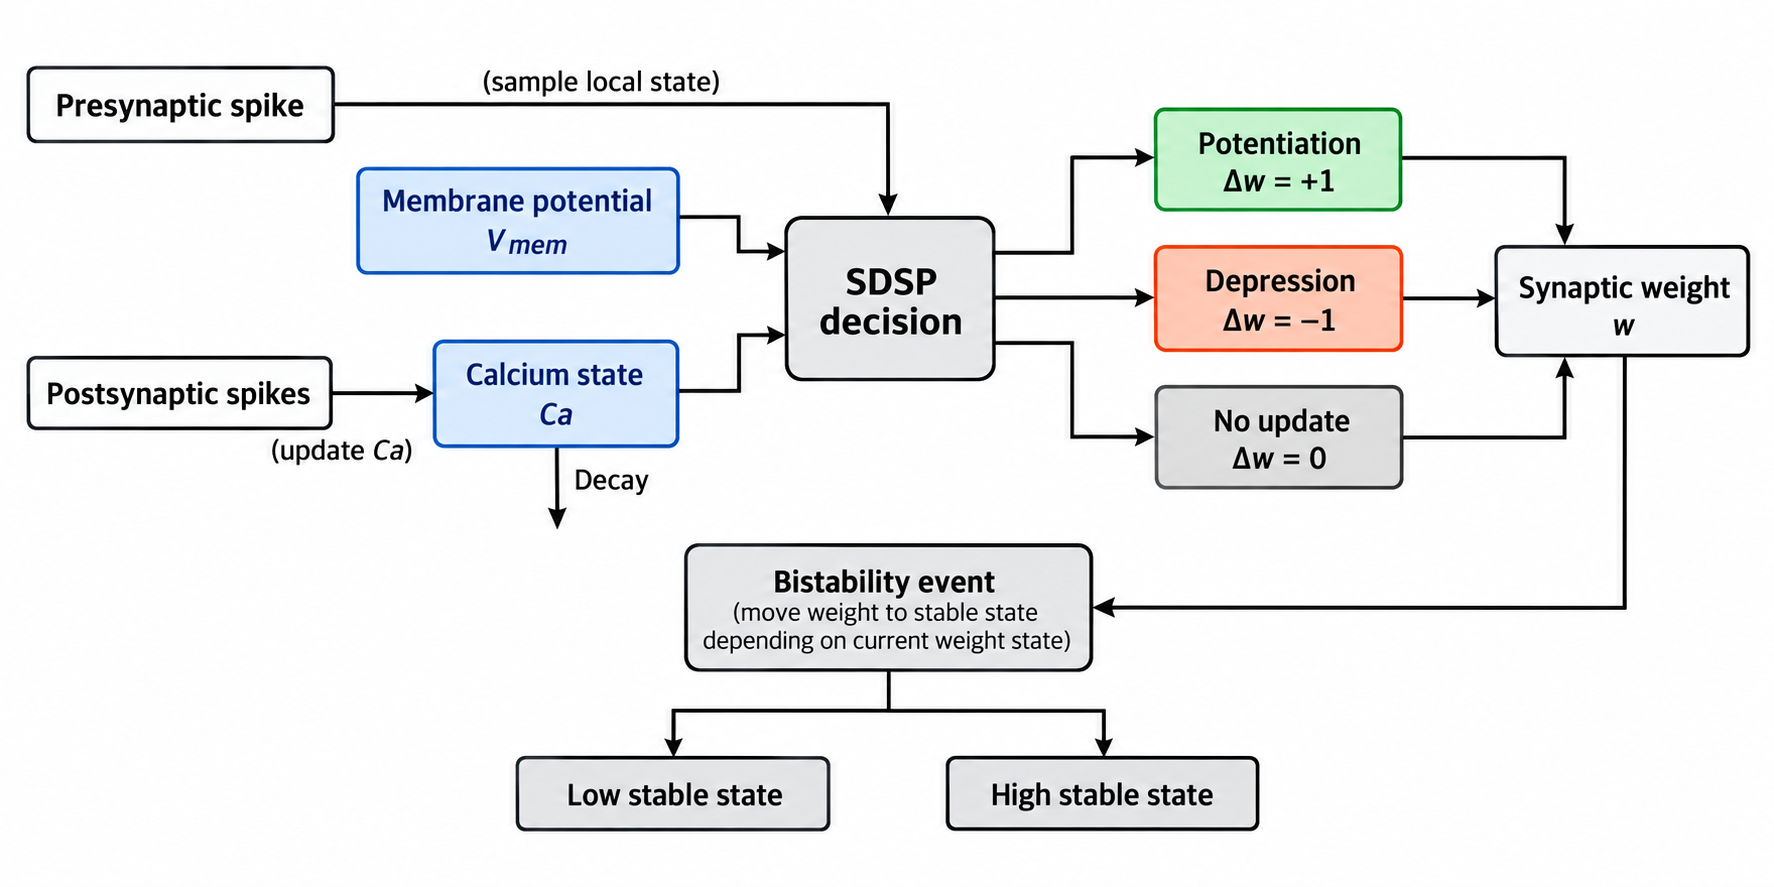
\includegraphics[width=.9\linewidth]{figures/sdsp_learning_rule.png}
	\caption{\gls{sdsp} Weight-Update Decisions and Bistability Mechanism}
	\label{fig:conceptual-operation-of-sdsp}
\end{figure}

\gls{sdsp} also includes a bistability mechanism. In the absence of a spike-driven update, the synaptic state gradually moves towards either a low or a high stable state. In the original formulation, this behaviour can be represented as

\begin{equation}
    \frac{\mathrm{d}w}{\mathrm{d}t}
    =
    \begin{cases}
        +\alpha, & w > \theta_w, \\
        -\beta,  & w \leq \theta_w
    \end{cases}
    \label{eq:synaptic-weight-drift}
\end{equation}

where \(\theta_w\) separates the two attraction regions, and \(\alpha\) and \(\beta\) determine the corresponding drift rates \cite{Brader2007}. This mechanism reduces the likelihood that a synaptic weight remains indefinitely in an unstable intermediate state.

In digital hardware, bistability can be implemented using periodic update events. When such an event occurs, the weight is incremented if it belongs to the upper region and decremented if it belongs to the lower region. The update continues until the weight reaches one of its numerical boundaries. With an unsigned binary representation, the most significant weight bit can be used to distinguish the two regions, avoiding a separate numerical comparison.

The \gls{sdsp} rule is suitable for hardware implementation because it requires only local state variables, threshold comparisons, and bounded weight increments or decrements. It does not require multiplication, global gradient computation, or the storage of precise presynaptic-to-postsynaptic timing differences. Digital processors such as ODIN have demonstrated that \gls{sdsp} can be implemented using time-multiplexed learning logic and on-chip writable synaptic memory \cite{Frenkel2019ODIN}.

In this work, the hardware-oriented \gls{sdsp} rule is adapted for integration with the \gls{snn} generated by Spiker+. The membrane potential and calcium state are represented using finite-width digital values, while the synaptic weights are modified using bounded integer updates. The exact numerical representation, threshold selection, control signals, and \gls{rtl} architecture are design-specific choices and are therefore presented later in Chapter \ref{sec:design_methodology} and Chapter \ref{sec:implementation}.

\section{FPGA-Based Neural Network Acceleration}
\label{subsec: fpga-based neural network acceleration}

\gls{fpga}s are reconfigurable integrated circuits whose hardware functionality can be defined after manufacturing. In contrast to processors that execute instructions sequentially, an \gls{fpga} allows application-specific datapaths and control structures to be implemented directly in hardware. This enables operations to be executed concurrently and makes \gls{fpga}s suitable for applications requiring low latency, deterministic timing, and adaptable hardware architectures.

\gls{fpga}s occupy a useful position between general-purpose processors and \gls{asic}s. \gls{cpu}s and \gls{gpu}s provide a convenient programming environment but execute applications on a predefined architecture. \gls{asic}s can offer higher efficiency, but their functionality is fixed after fabrication and their development requires considerable time and cost. \gls{fpga}s retain hardware-level parallelism while allowing the design to be modified and reprogrammed. These characteristics make them suitable for the development and evaluation of \gls{snn} accelerators \cite{Karamimanesh2025}.

A simplified overview of the main \gls{fpga} resources is shown in Figure \ref{fig:fpga-architecture-overview}. The main computational resources of an \gls{fpga} are configurable logic blocks. These blocks contain \gls{lut}s and \gls{ff}s that can be configured to implement combinational and sequential logic. \gls{lut}s can realize Boolean functions and small arithmetic operations, while \gls{ff}s store intermediate values and system states. Together, these resources can implement neuron update logic, comparators, counters, state machines, and learning-rule control circuits \cite{UG474}.

\begin{figure}[t]
	\centering
	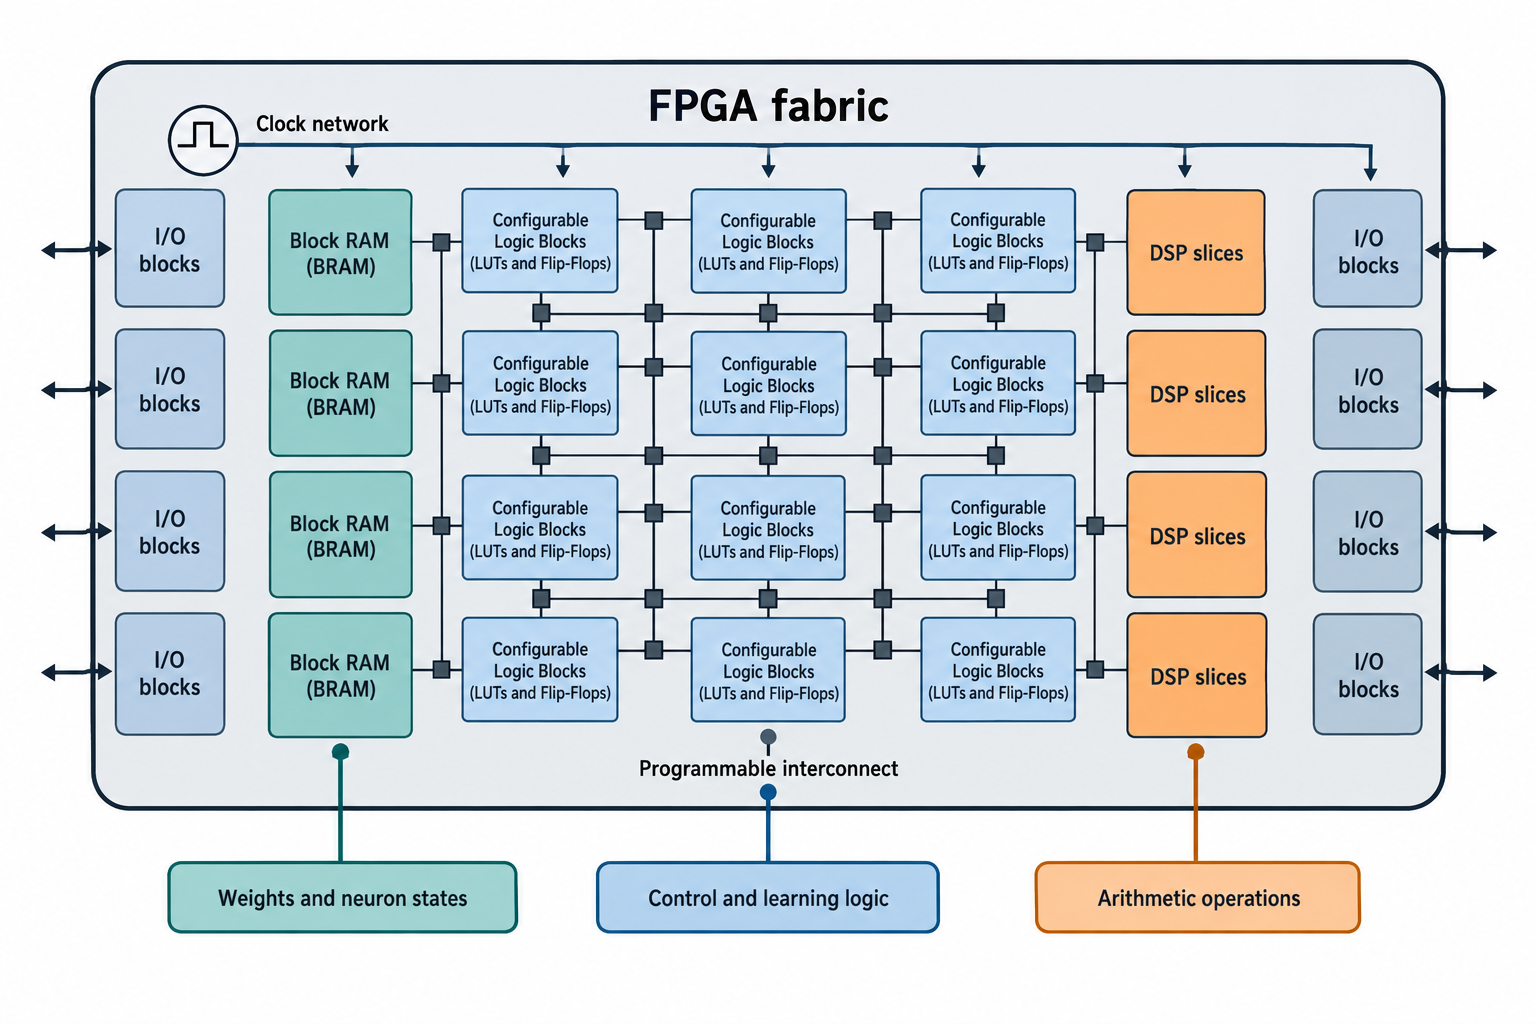
\includegraphics[width=.9\linewidth]{figures/fpga_architecture_overview.png}
	\caption{Principal \gls{fpga} Resources for \gls{snn} Acceleration}
	\label{fig:fpga-architecture-overview}
\end{figure}

Modern \gls{fpga}s also contain dedicated on-chip memory resources, commonly referred to as \gls{bram}. \gls{bram} provides larger and more structured storage than registers implemented using \gls{ff}s. In an \gls{snn} accelerator, it can be used to store synaptic weights, neuron membrane potentials, thresholds, input spikes, and intermediate network states. Since memory access often determines the performance and scalability of a neural-network accelerator, the organization of these memories is an important architectural decision \cite{UG473}.

Dedicated \gls{dsp} slices are provided for arithmetic operations such as multiplication, addition, and accumulation \cite{UG479}. They are particularly useful for traditional neural networks, which frequently require large numbers of multiply-accumulate operations. However, an \gls{snn} may require fewer multiplications because spikes are typically represented as binary events. Synaptic integration and local learning rules can often be implemented using additions, comparisons, and conditional updates. Depending on the selected neuron and learning models, these operations may therefore be implemented using configurable logic without requiring a large number of \gls{dsp} slices.

The parallel and configurable nature of an \gls{fpga} matches the computational characteristics of \gls{snn}s. Multiple neurons or synapses can be updated concurrently by allocating separate hardware resources to them. Alternatively, a smaller number of processing units can be reused across several neurons through time multiplexing. A fully parallel architecture can reduce processing latency but requires more hardware resources, whereas a time-multiplexed architecture reduces resource consumption at the cost of additional execution cycles. \gls{fpga}-based \gls{snn} design therefore involves a trade-off between resource utilization, latency, throughput, and supported network size.

An \gls{fpga} design is commonly described using a \gls{hdl} such as VHDL or Verilog. The \gls{rtl} description is first verified through simulation and then transformed into a hardware netlist through synthesis \cite{UG901}. During implementation, the synthesized logic is mapped to physical \gls{fpga} resources, placed on the device, and connected through the programmable routing network. After timing requirements have been verified, a configuration bitstream is generated and loaded onto the \gls{fpga} \cite{UG904}.

The main evaluation metrics for an \gls{fpga}-based neural network accelerator include the utilization of \gls{lut}s, \gls{ff}s, \gls{bram}, and \gls{dsp} slices. Timing characteristics such as maximum clock frequency, processing latency, and throughput are also important. In applications targeting embedded or edge systems, power consumption and energy efficiency may additionally be considered. These metrics allow different hardware architectures and resource-sharing strategies to be compared.

In this thesis, the Spiker+ framework is used as the basis for generating an \gls{fpga}-based \gls{snn} accelerator \cite{Carpegna2025}. The original inference-oriented architecture is extended with \gls{sdsp}-based online learning, which requires writable synaptic-weight storage and additional control logic for weight updates. \gls{fpga} technology makes it possible to integrate these functions into a customized hardware architecture while retaining the ability to modify the implementation. Its reconfigurable nature also motivated an assessment of whether learning functions could be exchanged at runtime. The following section introduces the \gls{dpr} concepts required for that assessment; Section \ref{subsec:dpr-applicability} explains why \gls{dpr} was excluded from the final implementation.

\section{Dynamic Partial Reconfiguration}
\label{subsec: dynamic partial reconfiguration}

\gls{fpga}s can be reprogrammed after manufacturing by loading configuration data into the device. In a conventional configuration process, a complete bitstream defines the functionality of the entire programmable logic. Loading a new full bitstream replaces the complete hardware design and normally interrupts all functions implemented in the \gls{fpga} fabric. Partial reconfiguration provides a more flexible alternative by modifying only a selected region of the device while leaving the remaining logic unchanged \cite{VipinFahmy2018}.

When partial reconfiguration is performed during system operation, it is commonly referred to as \gls{dpr}. AMD/Xilinx currently uses the term \gls{dfx} for this technology. Both terms describe the ability to exchange hardware functionality within a predefined region without reconfiguring the complete \gls{fpga} \cite{UG909}. In this thesis, the term \gls{dpr} is used as the general technological concept.

A \gls{dfx} design is divided into a static region and one or more reconfigurable partitions. The static region contains logic that remains configured throughout system operation, such as communication interfaces, memories, system controllers, and functions that must remain continuously available. A Reconfigurable Partition (RP) is a physically defined region of the \gls{fpga} reserved for dynamically replaceable functionality. The alternative hardware functions that can be loaded into this region are referred to as \glspl{rm} \cite{UG909}.

Each \gls{rm} may implement different functionality, but all modules assigned to the same \gls{rp} must use a compatible boundary interface. The interface defines the signals exchanged between the static logic and the reconfigurable module. The physical size of the \gls{rp} must also be sufficient for the largest \gls{rm} because every alternative module must be placed and routed within the same reserved \gls{fpga} region \cite{UG909,VipinFahmy2018}.

\begin{figure}[t]
	\centering
	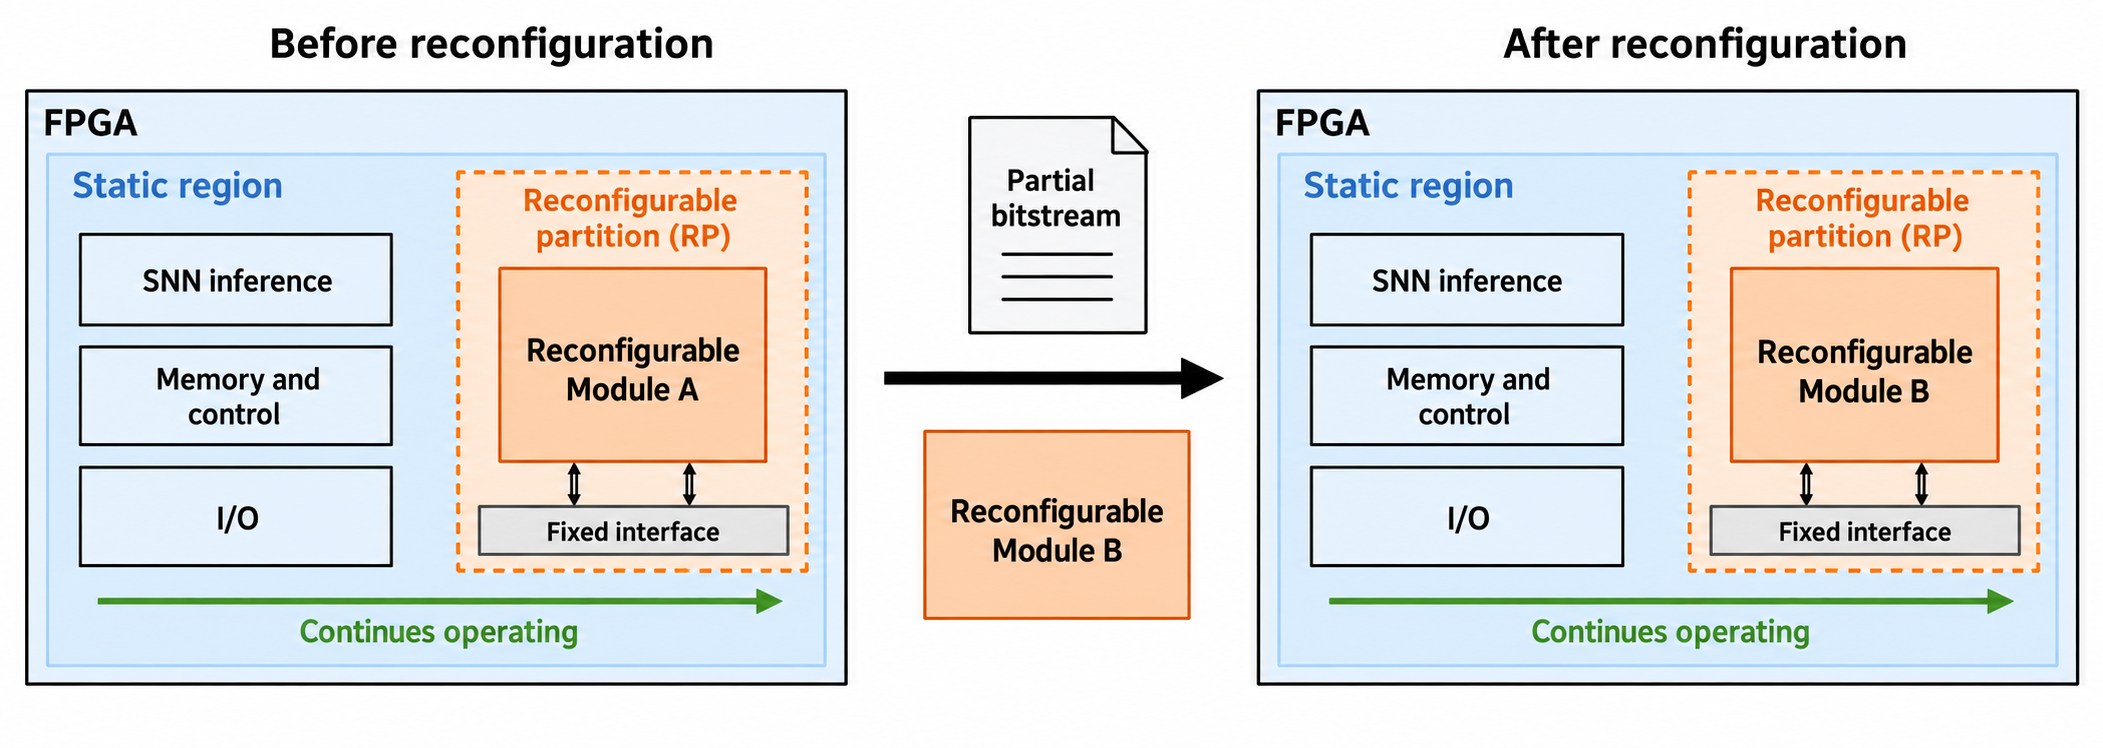
\includegraphics[width=.9\linewidth]{figures/dynamic_partial_reconfiguration.png}
	\caption{Basic Operating Principle of \gls{dpr}}
	\label{fig:basic-operating-principle-of-dpr}
\end{figure}

As shown in Figure \ref{fig:basic-operating-principle-of-dpr}, the initial \gls{fpga} configuration contains the static region and Reconfigurable Module A. To change the functionality, a partial bitstream containing the configuration data for Reconfigurable Module B is transferred to the \gls{fpga} configuration interface. Only the configuration frames associated with the \gls{rp} are modified. After the partial bitstream has been loaded, Module B occupies the same physical region and communicates with the static design through the same boundary interface.

The static region can continue operating during this process. However, the \gls{rp} itself is temporarily unavailable, and its output signals may be undefined while its configuration memory is being modified. Logic connected to the \gls{rp} must therefore not use these signals during reconfiguration. A decoupling mechanism can isolate the \gls{rp} boundary, while a controller stops new transactions, initiates the reconfiguration, waits for completion, and reconnects the new module afterwards \cite{UG909}. Therefore, \gls{dpr} does not guarantee that every function in the system continues without interruption; it allows the unaffected static logic to remain operational while the selected partition is temporarily replaced.

The \gls{dpr} implementation flow begins by separating the design hierarchy into static and reconfigurable components. An \gls{rp} is assigned to a physical region of the \gls{fpga} through floorplanning constraints, and each \gls{rm} is synthesized and implemented for this region. The static logic and \gls{rp} boundary must remain consistent across all configurations. The completed implementations are then verified for compatibility before full and partial bitstreams are generated \cite{UG909}.

A full bitstream is initially required to configure the complete device, including the static design and an initial \gls{rm}. During runtime, partial bitstreams are used to exchange only the content of the \gls{rp}. Depending on the \gls{fpga} platform, these bitstreams may be transferred through configuration interfaces such as the \gls{icap}, \gls{pcap}, JTAG, or another supported configuration path \cite{UG909}.

\section{Spiker+ Framework}
\label{subsec: spiker framework}

Spiker+ is an open-source framework for configuring, training, quantizing, and generating \gls{fpga} accelerators for \gls{snn} inference. It builds on the original Spiker accelerator, which introduced an FPGA-oriented, fixed-point architecture based on parallel neuron updates, sequential input-spike processing, and simplified \gls{lif} arithmetic \cite{Carpegna2022}. The original design demonstrated that these choices could reduce the hardware cost of an SNN accelerator, but it was developed primarily as a task-specific inference architecture. Spiker+ generalizes this foundation into a Python-controlled generation framework so that a user can describe an SNN at a higher abstraction level instead of manually constructing its complete \gls{rtl} hierarchy \cite{Carpegna2025}.

\subsection{Supported Design Space}

The built-in design space includes fully connected feedforward and recurrent networks. Its neuron library provides \gls{if}, first-order \gls{lif}, and second-order \gls{lif} models, each with either a fixed-reset or subtractive-reset implementation. A Python dictionary describes the selected network architecture, the number and size of its layers, the neuron model and parameters, the number of temporal processing steps, and the required feedback connections. The framework's network-builder module converts this description into a Python network object that is subsequently used by the training, optimization, and hardware-generation stages \cite{Carpegna2025}.

This separation between the high-level network description and the generated hardware is an important property of Spiker+. Network-level choices are expressed in Python, whereas implementation details such as control-unit instantiation, neuron datapaths, synchronization, and parameter initialization are produced by the generator. The framework is nevertheless not a general compiler for every possible SNN topology: its built-in generation flow targets the network structures and neuron models provided by its component library \cite{Carpegna2025}.

\subsection{Configuration and Generation Flow}

The complete Spiker+ configuration and generation process is illustrated in Figure \ref{fig:spikerplus-configuration-framework}. The flow consists of four principal stages: network construction, software training, numerical optimization, and VHDL generation \cite{Carpegna2025}.

\begin{figure}[t]
	\centering
	\makebox[\linewidth][c]{%
		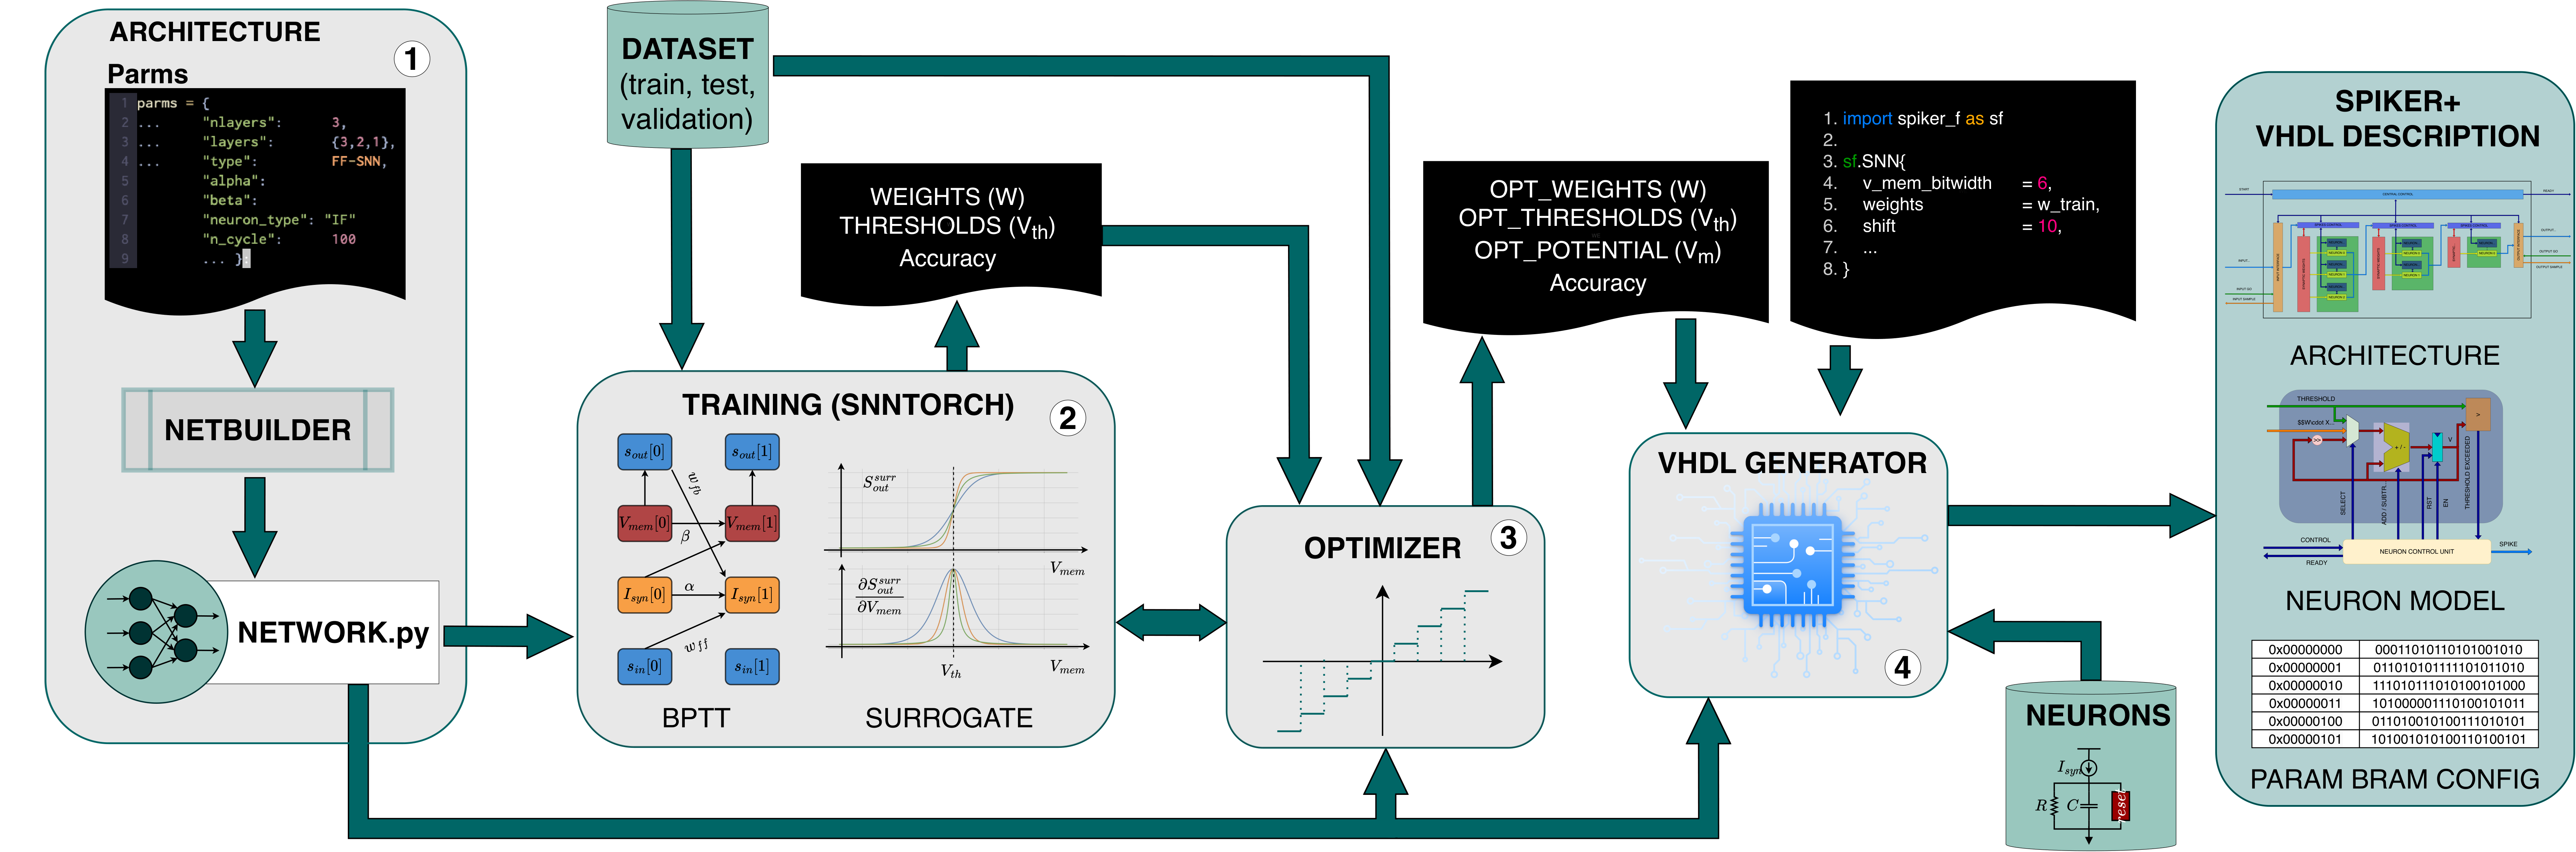
\includegraphics[width=1.10\linewidth]{figures/spikerplus_configuration_framework_original.png}%
	}
	\caption{Spiker+ Configuration, Optimization, and VHDL Generation Workflow \cite{Carpegna2025}}
	\label{fig:spikerplus-configuration-framework}
\end{figure}

In the first stage, the network builder creates the configured software model. The second stage trains this model using the framework's built-in integration with snnTorch and PyTorch. The training process produces the synaptic weights, firing thresholds, and other neuron parameters used during inference. Hardware-oriented approximations, such as restricting constant decay factors to shift-compatible values, can already be considered during training so that the software model reflects the arithmetic later used by the accelerator \cite{Carpegna2022,Carpegna2025}.

The third stage converts the floating-point training result into a signed \(N\)-bit fixed-point representation. Values outside the representable range are saturated, and the framework can evaluate several quantization widths to determine how reduced precision affects inference accuracy. This exploration is relevant because weight and membrane-potential widths influence both memory consumption and arithmetic cost. Reducing the weight width can also increase the number of weights obtained from an on-chip memory access, but the selected representation must retain sufficient numerical accuracy for the target network \cite{Carpegna2025}.

In the fourth stage, the VHDL generator translates the selected network object and its quantized parameters into synthesizable modules. It also produces parameter-initialization files for the synaptic memories and a file-driven testbench for simulation. The generated output is therefore not merely a parameter file for a fixed accelerator: it is a network-specific VHDL hierarchy that can subsequently be synthesized and implemented for the selected \gls{fpga} \cite{Carpegna2025}.

\subsection{Generated Hardware Architecture}

The generated accelerator follows three control levels. A Network Control Unit coordinates the temporal evolution of the complete network and synchronizes the layers and external interfaces. Each Layer Control Unit supplies the input spikes associated with one layer and waits for its neurons to complete the requested operation. At the lowest level, a Neuron Control Unit sequences the operations performed by its Neuron Datapath, including synaptic integration, leakage, threshold comparison, firing, and reset. Communication between adjacent blocks uses a two-signal \texttt{start}/\texttt{ready} handshake, which keeps the hierarchy modular and allows a controller to wait until all participating blocks have completed their current operation \cite{Carpegna2025}.

Spiker+ deliberately combines spatial parallelism with temporal reuse. All neurons in a layer can process the currently selected presynaptic input in parallel, whereas the individual inputs connected to that layer are supplied sequentially. The temporal steps of the spike train are also evaluated in sequence because each step depends on the evolving neuron state. This organization avoids instantiating one arithmetic datapath for every synapse while retaining parallel execution across the postsynaptic neurons. When no input spike is active in a time step, the layer controller can skip the otherwise unnecessary scan of its input connections, allowing sparse spike activity to reduce latency and switching activity \cite{Carpegna2022,Carpegna2025}.

The neuron datapaths exploit properties of the SNN model to simplify the arithmetic. Because a spike is binary, multiplying a synaptic weight by a spike becomes a conditional selection between zero and the weight. Fixed-point decay factors that are chosen as, or approximated by, powers of two allow constant multiplications to be replaced by shifts. These transformations reduce the need for general multipliers while preserving the neuron operations represented by the trained software model \cite{Carpegna2022,Carpegna2025}.

Synaptic weights are quantized and initialized from generated files. For the on-chip implementation, weights can be stored in \gls{bram}, whose independent memory blocks provide the bandwidth required to supply the weights of several neurons in parallel. Spiker+ also defines a synapse interface based on the same \texttt{start}/\texttt{ready} protocol, allowing an alternative memory organization to deliver the current weights before the layer proceeds. Using external memory can increase capacity, but the transfer required before each operation reduces the achievable accelerator speed \cite{Carpegna2025}.

The framework leaves the board-specific input and output implementation outside the generated neural core. Inputs may already be encoded as spike streams or may be converted from numerical data by a separate encoding block. At the output, the firing activity of the final layer can be accumulated and post-processed, for example by selecting the neuron with the largest spike count. The external interfaces must follow the accelerator's handshake protocol, but their concrete realization depends on the surrounding system \cite{Carpegna2025}. This boundary is used in Chapter \ref{sec:implementation}, where the generated network is connected to an AXI-based PYNQ data path.

\subsection{Relevance to This Thesis}

Spiker+ provides the baseline network hierarchy, neuron arithmetic, synchronization, and generated parameter memories used in this work. However, the framework version considered here targets inference with parameters obtained through offline training. Its generated synaptic weights are initialized for read access and remain fixed during network execution. Online learning consequently requires changes below the Python configuration level: the neuron state must be exposed to the learning rule, the excitatory memory must support runtime writes, and the layer schedule must retain the association between each update and its original synaptic address. Chapters \ref{sec:design_methodology} and \ref{sec:implementation} describe how these extensions are introduced while retaining the principal Spiker+ hierarchy and handshake structure.
